Classic {\em triangle centers} such as the incenter, barycenter, etc., are traditionally obtained via simple geometric constructions. Indeed, these can also be specified by special {\em triangle functions} which operate cyclically on sidelengths and/or angles \cite{kimberling1993_rocky}; see Appendix~\ref{app:triangle-centers}. Thousands appear on Kimberling's Encyclopedia  \cite{etc}. The list includes triangle functions which are rational, irrational, and more rarely, transcendental on sidelengths and/or angles. 

Consider the 1d family of 3-periodic orbits in the elliptic billiard (EB), Figure~\ref{fig:3-periodics}. The vertices are bisected by ellipse normals and the sides are tangent to a virtual confocal caustic; see Appendix~\ref{app:billiards} for a review. We have been drawn to this family because unexpectedly, the locus of the incenter is an ellipse and that of the {\em Mittenpunkt} $X_9$\footnote{The $X_k$ notation is after Kimberling \cite{etc}. The Mittenpunkt, was discovered by Nagel in 1836 as the point of concurrence of lines from the excenters through side midpoints \cite{mw}.} is the billiard center \cite{reznik2020-intelligencer}. Additionally, many other curious invariants have been detected and/or proved \cite{akopyan2020-invariants,bialy2020-invariants,reznik2020-invariants}. 

\begin{figure}
    \centering
    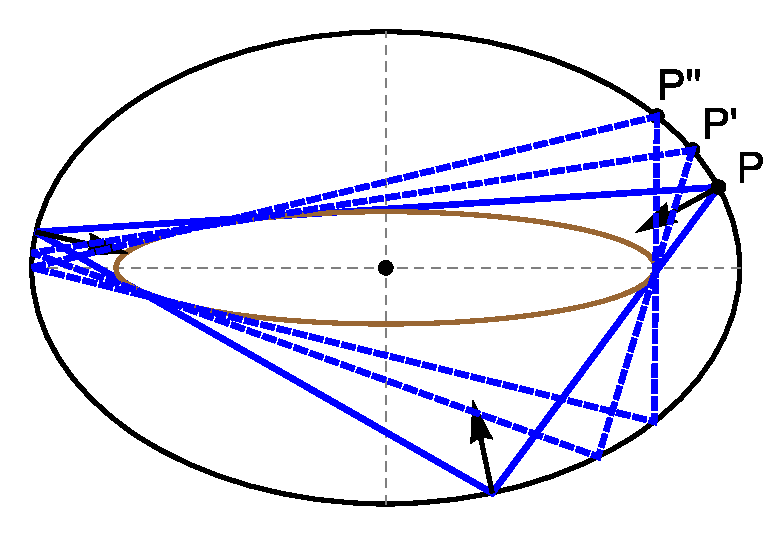
\includegraphics[width=.5\textwidth]{pics_1005_three_orbits_proofs.eps}
    \caption{Three 3-periodic orbits (one solid with vertex $P$ and two dashed with vertices $P'$, $P''$). The vertices are bisected by ellipse normals and the sides are dynamically tangent to a virtual confocal caustic (brown). Remarkably, the family conserves perimeter \cite{sergei91}. \href{https://bit.ly/38oncCD}{app}}
    \label{fig:3-periodics}
\end{figure}

In general, triangle centers sweep such curves as ellipses, quartics, sextics, etc., with or without self-intersections, etc.; see Figure~\ref{fig:incenter-loci}. The central question here is: given a triangle center, is it possible to predict its locus curve type over billiard 3-periodics based on the triangle function?

\begin{figure}
    \centering
    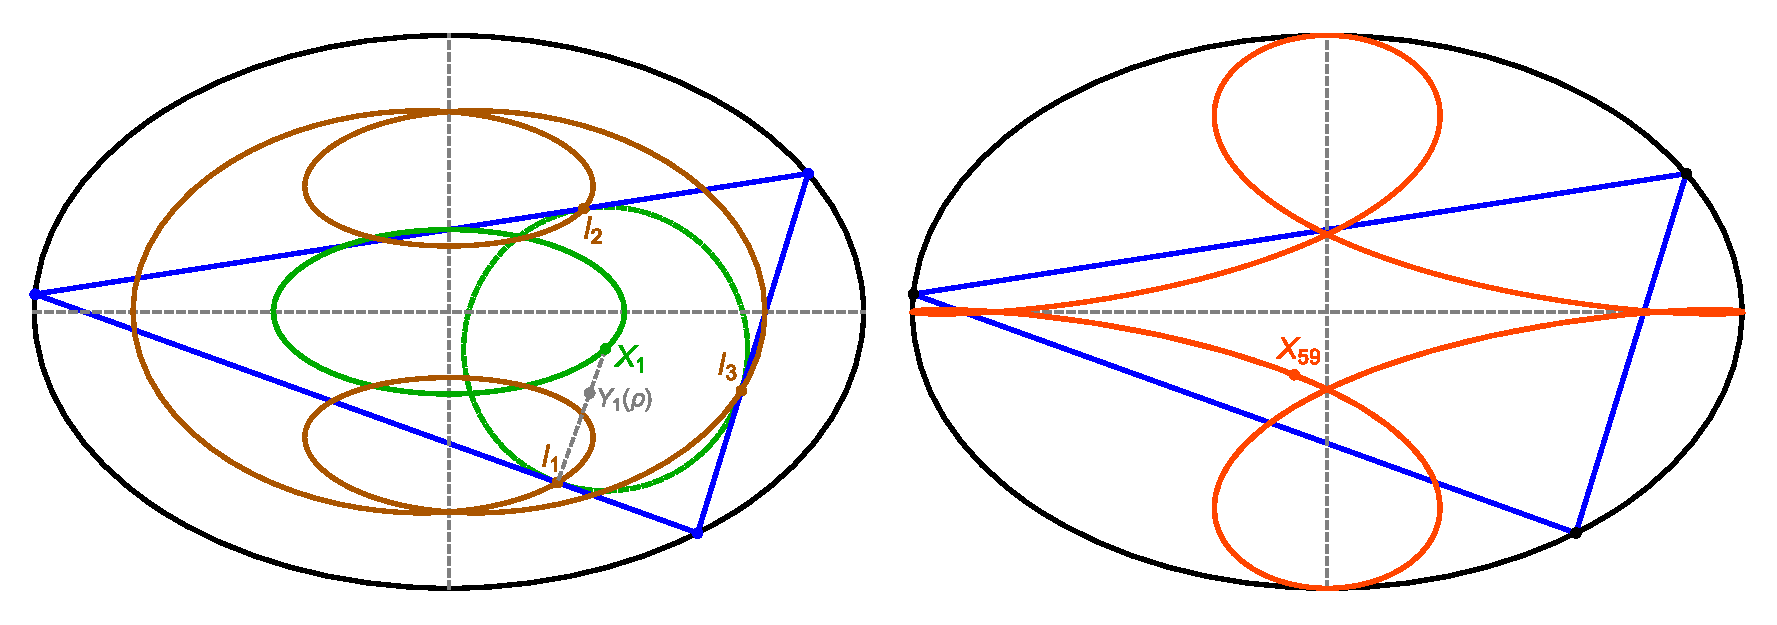
\includegraphics[width=\textwidth]{pics_1021_x1_x59}
    \caption{\textbf{Left}: A sample 3-periodic orbit (blue), the elliptic locus of the Incenter $X_1$ (green) and of that of the Intouchpoints $I_1,I_2,I_3$ (brown), the points of contact of the Incircle (dashed green) with the orbit sides. These produce a curve with two internal lobes whose degree is at least 6. $Y_1(\rho)$ is a convex combination of $X_1$ and $I_1$ referred to in Section~\ref{sec:triple-winding}. \href{https://bit.ly/3q4b0Nn}{app},  \href{https://youtu.be/BBsyM7RnswA}{Video 1}, \href{https://youtu.be/9xU6T7hQMzs}{Video 2}. \textbf{Right}: The locus of $X_{59}$ is a curve with four self-intersections. A vertical line epsilon away from the origin intersects the locus at 6 points. \href{https://bit.ly/3i4h6dX}{app}}
    \label{fig:incenter-loci}
\end{figure}

\subsection*{Main Results}

We present a method to rigorously verify if the locus of given triangle center is an ellipse or not. We apply it to the first 100 Centers listed in \cite{etc}, finding that 29 are elliptic. We have derived explicit expressions for their axes \cite{garcia2021-ellipses-web}.

We prove (Theorem~\ref{thm:rational-center}) that when a triangle center is rational on the sidelengths, the locus (elliptic or not) will be algebraic. We also describe a method based on the theory of resultants which computes the irreducible polynomial in two variables, whose zero set is the Zariski Closure \cite{cox2005-AG} of the locus. From wide experimentation, no irrational triangle function has yet produced an elliptic locus, so it is likely that for a locus to be elliptic its triangle function must be rational.

We also consider the curious case of the Symmedian Point $X_6$, whose locus closely approximates an ellipse but it is actually a quartic, which we derive explicitly. Interestingly, its triangle function is rational and one of the simplest in \cite{etc}; see Table~\ref{tab:center-trilinears}.

For the general case of triangle function to locus type, we still lack a theory.

\subsection*{Related Work}

Odehnal extensively studied loci of triangle centers over the poristic triangle family \cite{odehnal2011-poristic}. Our early experimental result that the locus of the Incenter $X_1$ of billiard 3-periodics is an ellipse was subsequently proven \cite{olga14,garcia2019-incenter}. Proofs soon followed for the ellipticity of both $X_2$ \cite{sergei2016-com} and $X_3$ \cite{corentin19,garcia2019-incenter}; see Figures \ref{fig:non-elliptic-vertex} and \ref{fig:x12345-feuer-combo} in Appendix~\ref{app:early}.

\subsection*{Outline}

Our main methods appear in Sections~\ref{sec:loci_geom} and \ref{sec:algebraic}. We conclude in Section~\ref{sec:conclusion} with a list of questions and interesting links and videos. The Appendices contain supporting material. Most figures contain clickable links to relevant videos and/or the experiment displayed on our browser-based \href{https://dan-reznik.github.io/ellipse-mounted-loci-p5js}{app} \cite{darlan2020-ellipse-mounted}.
